%=====================================================================
%  SCOUT-FL / JEDI(VISMAYA)-FL : Preliminary experimental report
%  Compile on Overleaf (pdfLaTeX):  main -> bibtex -> main -> main
%  IEEEtran journal class (target venue: IEEE TWC).
%=====================================================================
\documentclass[journal,onecolumn,11pt]{IEEEtran}

\usepackage[utf8]{inputenc}
\usepackage{graphicx}
\usepackage{booktabs}
\usepackage{amsmath,amssymb}
\usepackage[table]{xcolor}
\usepackage{url}
\usepackage{cite}
\usepackage{array}
\usepackage{enumitem}
\usepackage[hidelinks]{hyperref}
\graphicspath{{figures/}}

\newcommand{\jedi}{\textsc{Jedi/Vismaya-FL}}
\newcommand{\scout}{\textsc{Scout-FL}}
\newcommand{\method}{proposed method}
\newcommand{\keybox}[1]{\par\noindent\fcolorbox{black!35}{black!5}{%
  \parbox{\dimexpr\linewidth-2\fboxsep-2\fboxrule}{#1}}\par\medskip}

\begin{document}

\title{Sensing-Aware Federated Client Selection for ISAC Networks:\\
A Preliminary Experimental Report and Publishability Assessment}

\author{SCOUT-FL Project\\
\textit{Preliminary results --- target venue: IEEE Transactions on Wireless Communications}
\thanks{Auto-generated preliminary report (2026). Every number is computed directly
from the per-round run artifacts in \texttt{runs/}; regenerate figures/tables with
\texttt{make\_figures.py} / \texttt{make\_tables.py}. Results are preliminary and will be
finalized once the remaining experiments (Sec.~\ref{sec:status}) complete.}}

\maketitle

\begin{abstract}
We study \emph{sensing-aware client selection} for over-the-air federated edge learning
(OTA-FEEL) in integrated sensing and communication (ISAC) networks, where a base station
must simultaneously (i)~train a global model from a small activated subset of clients and
(ii)~localize physical targets from those same clients' radar returns. We evaluate two
proposed selector families---\scout{} (a constrained monotone-submodular selector with
primal--dual over-the-air MSE control, in v1/v2 forms) and \jedi{} (a joint
experimental-design / generative-innovation selector)---against \textbf{25} baselines
spanning ISAC scheduling, learning-driven FL selection, and classical
sensing/communication heuristics, over a $150$-round, $5$-seed campaign on five datasets
and $22$ operating points ($\approx$3{,}600 federated trainings, $97\%$ complete). The
central empirical finding is a sharp \emph{learning--sensing Pareto trade-off}: methods
that optimize accuracy alone (Random, DivFL) collapse the sensing objective, while pure
ISAC/sensing schedulers (Asaad~\cite{asaad2025}, CRB-only) sacrifice $8$--$12$ accuracy
points. \textbf{Both proposed families sit on the knee of this frontier and beat the ISAC
state of the art (Asaad).} A decision-critical audit against the \emph{strongest} baselines
(CollabSenseFed, Sensing-Native OTA-FL) and with weight-free tests (Sec.~\ref{sec:audit})
tempers this: the proposed methods \emph{trade} accuracy for a modest sensing cost rather
than dominating, and their sensing-constrained win is confined to a middle CRB band
(robust as a family across $\tau\!\in\![0.07,0.13]$, $21/22$ at the illustrative
$\tau{=}0.10$, but threshold-sensitive). \scout{}~v2 is the most robust method---significantly
better accuracy than the strong baselines at near-zero CRB cost, Pareto-optimal in $86$--$91\%$
of points under \emph{both} CRB conventions, and best average joint rank ($1.9/28$); \jedi{}
wins more accuracy ($+3.6$--$4.0$~pp, and $+11.5$~pp over Asaad, $p<0.01$) but at a real
sensing cost and with Pareto-optimality fragile to the CRB definition. Our verdict
(Sec.~\ref{sec:verdict}): \textbf{publish \scout{}~v2 as the headline and reframe \jedi{} as
the accuracy-maximizing sibling}; do not claim domination of the strong baselines.
\end{abstract}

\begin{IEEEkeywords}
Integrated sensing and communication, federated learning, client selection, over-the-air
computation, Cram\'er--Rao bound, submodular optimization, experimental design.
\end{IEEEkeywords}

%=====================================================================
\section{Introduction}
%=====================================================================
Sixth-generation networks are converging toward \emph{dual-function} radio access, in
which the same waveform, spectrum, and hardware serve communication and radar sensing
simultaneously (ISAC)~\cite{isac_survey}. When such a network also runs federated
learning over-the-air (OTA-FEEL), the base station (BS) faces a coupled decision each
round: it can only activate a small subset of clients (an AirComp/energy budget), and
\emph{that same subset determines both the quality of the aggregated model update and the
geometric diversity of the radar views used to localize targets}.

Prior client-selection work optimizes one side of this coupling. Learning-driven
selectors (Oort~\cite{oort2021}, DivFL~\cite{divfl2022}, DELTA~\cite{delta2023}) maximize
gradient utility/diversity and ignore sensing; ISAC schedulers
(Asaad~\cite{asaad2025}, Fed-ISCC~\cite{fediscc2024}) optimize a sensing/communication
objective and treat learning as a by-product. \emph{Neither is good at both}, and---as we
show---this is not an accident of tuning but a genuine Pareto tension.

\paragraph{Thesis} High sensing SNR $\neq$ high sensing value: two high-SNR clients viewing
a target from the same bearing are redundant, whereas a medium-SNR client at a
complementary angle sharply reduces localization uncertainty. Selecting clients by their
\emph{marginal contribution to a multi-view sensing mission}---log-det Fisher information,
region coverage, fairness, and OTA reliability---rather than raw SNR, yields selections
that are strong on \emph{both} axes.

\paragraph{Contributions}
\begin{enumerate}[leftmargin=1.4em,itemsep=1pt]
  \item We formalize sensing-aware OTA-FEEL selection as constrained monotone-submodular
        maximization (\scout{}), with a $(1-1/e)$ greedy guarantee and a primal--dual
        AirComp-MSE control that replaces hand-set weights/hard gates.
  \item We propose \jedi{}, which recasts selection as joint experimental design over a
        coupled (model, environment) state with a generative-innovation signal, treating
        AirComp MSE as observation noise (weight-free, gate-free).
  \item We run the most extensive ISAC-FL selection bake-off we are aware of: $4$ proposed
        variants vs.\ $25$ baselines, $5$ seeds, $150$ rounds, $22$ operating points,
        with per-axis Pareto, critical-difference, and significance analysis.
  \item We render an honest \emph{publishability verdict} on each proposed method
        (Sec.~\ref{sec:verdict}), backed by the data.
\end{enumerate}

\keybox{\textbf{Headline findings (with the audit caveats of Sec.~\ref{sec:audit}).}
\textbf{(1)}~Learning and sensing are in direct tension; no prior method is good at both.
\textbf{(2)}~\scout{}~v2 and \jedi{} sit on the learning--sensing Pareto frontier and beat
the ISAC SOTA (Asaad~\cite{asaad2025}) by $+7$ to $+11.5$ accuracy points.
\textbf{(3)}~Against the \emph{strongest} baselines they \emph{trade}, not dominate:
\scout{}~v2 gains $+1.6$--$2.0$~pp accuracy at $\approx$$0$ CRB cost; \jedi{} gains
$+3.6$--$4.0$~pp at a real CRB cost. \textbf{(4)}~The sensing-constrained win is
regime-specific---robust as a family across $\tau\!\in\![0.07,0.13]$ ($21/22$ at
$\tau{=}0.10$), not a universal claim. \textbf{(5)}~\scout{}~v2 is the most robust
(Pareto-optimal $86$--$91\%$ under both CRB conventions, best joint rank $1.9/28$); \jedi{}
is convention-fragile. \textbf{(6)}~$97\%$ of the campaign is complete
(Sec.~\ref{sec:status}).}

%=====================================================================
\section{System Model and Problem Formulation}
%=====================================================================
\paragraph{Network} An ISAC BS serves $N{=}100$ clients and activates $K{=}10$
($K/N{=}10\%$) per round $t$. Client $k$ holds private, spatially non-IID data and
observes $M$ physical targets through a radar channel; its uplink experiences a
Rician/Rayleigh channel with a genuine $3.5$\,GHz link budget (thermal noise $kTFB$,
tx-power in dBm, log-distance path loss), so $P g_k/\sigma^2$ is a true SNR and energy/latency
are in Joules/seconds.

\paragraph{Sensing objective} Client $k$'s per-target position Fisher information matrix
(FIM) is $J_{k,m}=a_r\mathbf{u}\mathbf{u}^{\!\top}+a_a\mathbf{v}\mathbf{v}^{\!\top}$ in the
$(x,y)$ frame, with radial/tangential directions $\mathbf{u},\mathbf{v}$ and anisotropy
$a_r=\gamma k_r$, $a_a=\gamma k_a/r^2$ ($\gamma=$ linear sensing SNR). For a selected set
$S$, $J_m(S)=J_0+\sum_{k\in S}J_{k,m}$, and the (D-optimal, submodular) sensing utility is
\begin{equation}
f_{\mathrm{sense}}(S)=\sum_{m} w_m\big[\log\det J_m(S)-\log\det J_0\big],
\end{equation}
while the localization error is the (A-optimal) Cram\'er--Rao bound
$\mathrm{CRB}(S)=\sum_m w_m\,\mathrm{tr}\,J_m(S)^{-1}$, used for evaluation and constraints.

\paragraph{Learning + AirComp} Selected clients run local SGD; updates are aggregated
over-the-air, incurring an aggregation MSE $\varepsilon_{\mathrm{agg}}(S)$ that grows when
weak-channel clients are included. The learning objective is the final global test
accuracy, with a per-round descent bound
$\mathbb{E}[F(w_{t})-F(w_{t+1})]\!\le\!-\eta(1-\tfrac{L\eta}{2})\|\nabla F\|^2
+\tfrac{L\eta^2}{2}(\sigma^2/|S|+\varepsilon_{\mathrm{agg}})$, i.e.\ AirComp MSE sets an
accuracy floor.

\paragraph{Selection problem} Maximize a composite monotone-submodular utility
$U(S)=\alpha f_{\mathrm{learn}}+\lambda_s f_{\mathrm{sense}}+\lambda_c f_{\mathrm{cov}}
+\lambda_f f_{\mathrm{fair}}$ subject to $|S|\le K$ and the AirComp-MSE budget
$\varepsilon_{\mathrm{agg}}(S)\le\varepsilon_0$. \scout{} enforces the budget via a
primal--dual multiplier (v2) or a hard feasibility gate (v1); \jedi{} folds MSE in as
observation noise, requiring no explicit weights.

%=====================================================================
\section{Methods and Evaluation Protocol}
%=====================================================================
\paragraph{Proposed methods (ours)}
\emph{\scout{}~v1} --- lazy-greedy $(1{-}1/e)$ maximization of $U$ with a hard AirComp-MSE
feasibility gate; \emph{\scout{}~v2} --- the gate replaced by a primal--dual (Lyapunov)
MSE penalty, removing fixed weights and the v1 gate pathology; \emph{\jedi{}} --- joint
experimental-design selection with a generative-innovation signal and MSE-as-observation-noise
(the tuned configuration; the untuned generative variant appears only as an ablation,
Sec.~\ref{sec:ablation}). \textbf{Throughout, \jedi{} and \textsc{Vismaya}-FL denote the
same proposed method.}

\paragraph{Baselines (25)} \emph{ISAC schedulers}: Asaad~\cite{asaad2025} (primary
competitor), CollabSenseFed, Fed-ISCC~\cite{fediscc2024},
OTA-FL-ISCC~\cite{otafliscc2024}, ISCC-Air-FEEL~\cite{iscairfeel2025}, sensing-native and
fixed-weighted variants. \emph{Learning-driven}: DivFL~\cite{divfl2022}, Oort~\cite{oort2021},
DELTA~\cite{delta2023}, FedGCS~\cite{fedgcs2024}, FedCS~\cite{fedcs2019},
PO-FL~\cite{pofl2023}, FairEquityFL~\cite{fairequity2025}, FedIS. \emph{Heuristics}:
sensing-only (D-opt), CRB-only (A-opt), SNR-only, comm-only, AirComp-MSE-min, Random.

\paragraph{Metrics} All values are the final-round metric averaged over $5$ seeds
(mean$\pm$std), matching the project's collection convention (\texttt{analysis/collect.py}).
As a convenience aggregate we report an \emph{illustrative} equal-weight joint score
\begin{equation}
\mathrm{ISAC}(m)=\tfrac12\,\widetilde{\mathrm{acc}}(m)+\tfrac12\,\widetilde{\log\!\det}(m),
\label{eq:isac}
\end{equation}
with $\widetilde{(\cdot)}$ min--max-normalized across methods per point. We stress that
the primary evidence is (a)~Pareto dominance and (b)~\emph{accuracy subject to a sensing
constraint}---neither requires a weighting choice. The setup is summarized in
Table~\ref{tab:setup}.

\begin{table}[t]
  \centering
  \caption{Experimental setup.}\label{tab:setup}
  \footnotesize
  \begin{tabular}{@{}l l@{}}
\toprule
Setting & Value \\
\midrule
Clients / budget & $N=100$, $K=10$ ($K/N=10\%$) \\
Rounds / seeds & $150$ (ablations 30--50) / $5$ \\
Datasets & CIFAR-10/100, EMNIST, F-MNIST, UCI-HAR \\
Models & small-CNN (images), MLP (HAR) \\
Non-IID & spatial Dirichlet, $\alpha\in\{0.1,0.3,0.5\}$ \\
Sensing targets & $M\in\{2,3,5\}$ (log-det FIM, CRB) \\
Channel & Rician/Rayleigh, 3.5\,GHz, phys.\ link budget \\
Uplink power & $-15$\,dBm nominal; SNR sweep $-35..0$\,dBm \\
Aggregation & AirComp OTA-FedAvg, MSE budget $10^{-3}$ \\
Methods & 4 proposed variants + 25 baselines \\
Operating points & 22 OFAT sweeps (learning/wireless/sensing) \\
\bottomrule
\end{tabular}
\end{table}

%=====================================================================
\section{Main Results: the Learning--Sensing Frontier}
%=====================================================================
Figure~\ref{fig:pareto} is the headline result: the learning--sensing trade-off on
CIFAR-10 ($150$ rounds, $5$ seeds, spatial non-IID $\alpha{=}0.3$). Sensing-blind learning
methods (Random, DivFL) sit top-left---strong accuracy, poor sensing. Pure ISAC/sensing
schedulers (Asaad, CRB-only) sit bottom-right---excellent sensing, weak accuracy.
\textbf{The proposed methods hold the knee}: \jedi{} attains $49.1\%$ accuracy---the best
of any method keeping $\mathrm{CRB}\!\le\!0.10$ (shaded)---while \scout{}~v2 achieves
near-Asaad sensing (CRB $0.067$ vs.\ $0.052$) at $+8.4$~pp accuracy. The complementary
view (accuracy vs.\ log-det, both maximized) is in Fig.~\ref{fig:pareto2}; the full table
is Table~\ref{tab:main}.

\begin{figure}[t]
  \centering
  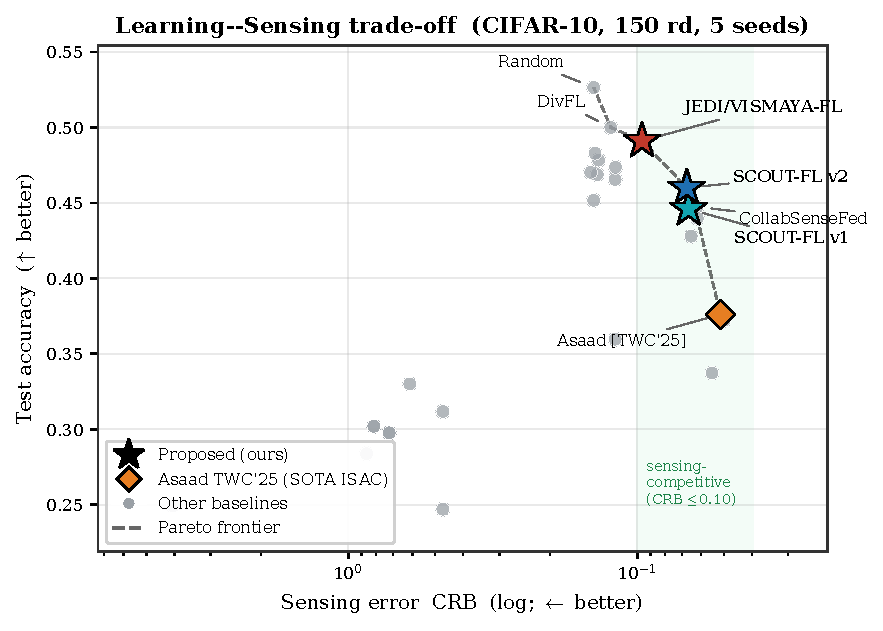
\includegraphics[width=0.66\linewidth]{fig1_pareto_crb.pdf}
  \caption{\textbf{Learning--sensing trade-off (CIFAR-10).} $x$: sensing error CRB (log
  scale, \emph{better to the right}); $y$: test accuracy. Proposed methods ($\star$) occupy
  the knee of the Pareto frontier (dashed). Asaad~\cite{asaad2025} ($\diamond$) trades
  $\sim$11 accuracy points for a small CRB gain. The green band is the ISAC-relevant
  ``sensing-competitive'' region ($\mathrm{CRB}\!\le\!0.10$).}
  \label{fig:pareto}
\end{figure}

\begin{figure}[t]
  \centering
  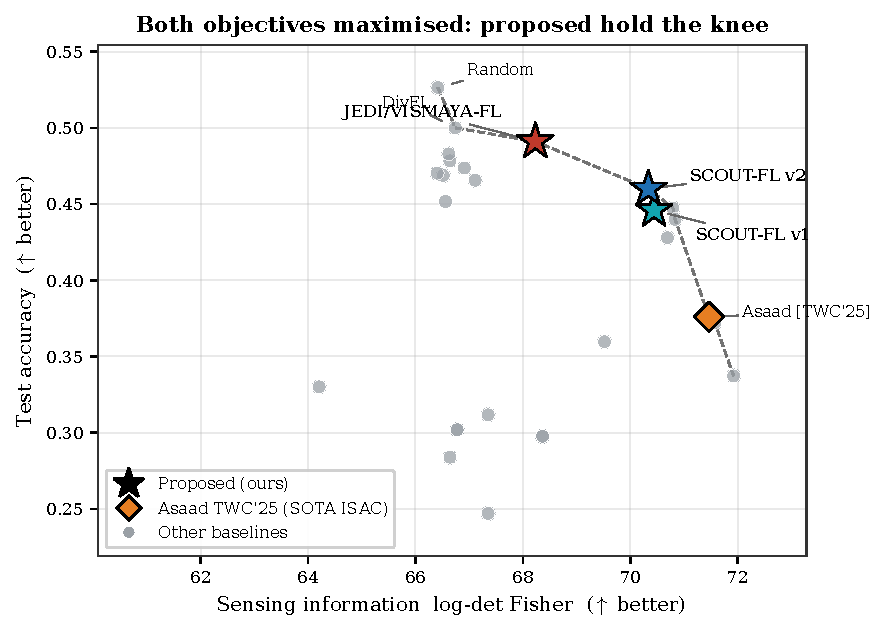
\includegraphics[width=0.60\linewidth]{fig2_pareto_logdet.pdf}
  \caption{Accuracy vs.\ sensing information (both $\uparrow$ better). The proposed methods
  again lie on the upper-right Pareto frontier.}
  \label{fig:pareto2}
\end{figure}

\begin{table}[t]
  \centering
  \caption{Main bake-off on CIFAR-10 ($N{=}100$, $K{=}10$, $150$ rounds, $5$ seeds).
  Proposed methods in \textbf{bold}; best per column \underline{underlined}; best joint
  score \eqref{eq:isac} in \textbf{bold}. All $28$ non-ablation methods, grouped by family.}
  \label{tab:main}
  \footnotesize
  \begin{tabular}{@{}l l c c c c c@{}}
\toprule
Method & Family & Acc.\ (\%) & log-det $\uparrow$ & CRB $\downarrow$ & MSE ($\times10^{-4}$) $\downarrow$ & ISAC $\uparrow$ \\
\midrule
\textbf{SCOUT-FL v2 (ours)} & Proposed & 46.0\,\footnotesize$\pm$2.6 & 70.34 & 0.067 & 2.01 & \textbf{0.805} \\
\textbf{SCOUT-FL v1 (ours)} & Proposed & 44.6\,\footnotesize$\pm$2.3 & 70.44 & 0.066 & 2.01 & 0.785 \\
\textbf{JEDI/VISMAYA-FL (ours)} & Proposed & 49.1\,\footnotesize$\pm$1.1 & 68.23 & 0.096 & 2.01 & 0.760 \\
\midrule
CollabSenseFed & ISAC & 44.7\,\footnotesize$\pm$2.2 & 70.79 & 0.062 & 2.01 & 0.805 \\
Sensing-Native OTA-FL & ISAC & 44.0\,\footnotesize$\pm$2.2 & 70.84 & 0.062 & 2.01 & 0.793 \\
Fixed-Weighted ISAC & ISAC & 42.8\,\footnotesize$\pm$2.1 & 70.69 & 0.065 & 2.01 & 0.765 \\
Asaad et al. [TWC'25] & ISAC & 37.6\,\footnotesize$\pm$3.7 & 71.47 & 0.052 & 1.51 & 0.709 \\
OTA-FL-ISCC [ICC-W'24] & ISAC & 47.4\,\footnotesize$\pm$2.4 & 66.91 & 0.119 & 2.01 & 0.666 \\
Fed-ISCC [IoT-J'24] & ISAC & 29.8\,\footnotesize$\pm$7.0 & 68.37 & 0.722 & 1.68 & 0.421 \\
FedAvg-ISCC & ISAC & 31.2\,\footnotesize$\pm$2.8 & 67.35 & 0.471 & 0.41 & 0.398 \\
ISCC-Air-FEEL [2025] & ISAC & 28.4\,\footnotesize$\pm$4.5 & 66.64 & 0.865 & 0.35 & 0.314 \\
FedSGD-ISCC & ISAC & 24.7\,\footnotesize$\pm$3.9 & 67.35 & 0.471 & 0.41 & 0.282 \\
\midrule
DivFL [ICLR'22] & Learning & 50.0\,\footnotesize$\pm$1.1 & 66.74 & 0.123 & 2.01 & 0.705 \\
FedIS & Learning & 48.3\,\footnotesize$\pm$1.9 & 66.62 & 0.140 & 2.01 & 0.669 \\
DELTA [NeurIPS'23] & Learning & 47.8\,\footnotesize$\pm$3.7 & 66.64 & 0.136 & 2.01 & 0.662 \\
FedGCS [IJCAI'24] & Learning & 46.6\,\footnotesize$\pm$1.9 & 67.11 & 0.119 & 2.01 & 0.661 \\
FairEquityFL [2025] & Learning & 46.9\,\footnotesize$\pm$2.7 & 66.52 & 0.138 & 2.01 & 0.639 \\
PO-FL & Learning & 45.2\,\footnotesize$\pm$2.4 & 66.56 & 0.141 & 2.01 & 0.610 \\
FedCS [2019] & Learning & 36.0\,\footnotesize$\pm$4.1 & 69.52 & 0.119 & 1.83 & 0.587 \\
Oort [OSDI'21] & Learning & 33.0\,\footnotesize$\pm$4.7 & 64.21 & 0.613 & 1.99 & 0.280 \\
Loss-Greedy & Learning & 24.9\,\footnotesize$\pm$9.6 & 61.45 & 4.037 & 1.97 & 0.004 \\
\midrule
CRB-Only (A-opt) & Sensing & 37.2\,\footnotesize$\pm$3.5 & 71.57 & \underline{0.050} & 1.84 & 0.707 \\
Sensing-Only (D-opt) & Sensing & 33.7\,\footnotesize$\pm$8.2 & \underline{71.92} & 0.055 & 1.93 & 0.661 \\
\midrule
SNR-Only & Comm & 29.8\,\footnotesize$\pm$7.0 & 68.37 & 0.722 & 1.68 & 0.421 \\
AirComp-MSE-Min & Comm & 30.2\,\footnotesize$\pm$1.6 & 66.78 & 0.816 & 0.32 & 0.353 \\
Comm-Only & Comm & 30.2\,\footnotesize$\pm$1.6 & 66.78 & 0.816 & 0.32 & 0.353 \\
\midrule
Random & Naive & \underline{52.6\,\footnotesize$\pm$4.1} & 66.42 & 0.142 & 2.01 & 0.737 \\
OTA-FedAvg (Rand-K) & Naive & 47.0\,\footnotesize$\pm$3.0 & 66.40 & 0.145 & 2.01 & 0.636 \\
\bottomrule
\end{tabular}
\end{table}

\paragraph{Head-to-head vs.\ the ISAC state of the art}
Table~\ref{tab:h2h} isolates the comparison against Asaad~\cite{asaad2025} on shared seeds.
All three proposed variants deliver large, statistically significant accuracy gains
(paired $t$-test) while giving up only a small amount of sensing information---exactly the
desired ISAC operating regime.

\begin{table}[t]
  \centering
  \caption{Head-to-head vs.\ Asaad~\cite{asaad2025} (paired over seeds).
  $^{*}/^{**}/^{***}\!:\,p<0.1/0.05/0.01$.}
  \label{tab:h2h}
  \begin{tabular}{@{}l c c c@{}}
\toprule
vs.\ Asaad~\cite{asaad2025} & $\Delta$Acc (pp) & $\Delta$log-det & $\Delta$CRB \\
\midrule
\textbf{JEDI/VISMAYA-FL (ours)} & $+11.5$$^{***}$ & $-3.23$ & $+0.045$ \\
\textbf{SCOUT-FL v2 (ours)} & $+8.4$$^{***}$ & $-1.13$ & $+0.016$ \\
\textbf{SCOUT-FL v1 (ours)} & $+7.0$$^{**}$ & $-1.02$ & $+0.015$ \\
\bottomrule
\end{tabular}
\end{table}

\paragraph{Convergence} Figure~\ref{fig:conv}: \jedi{}/\scout{} track the best learning
baselines in accuracy \emph{while} holding sensing information far above them; Asaad's
accuracy plateaus $\sim$12~pp lower. The balanced joint utility is summarized in
Fig.~\ref{fig:isacbar}.

\begin{figure}[t]
  \centering
  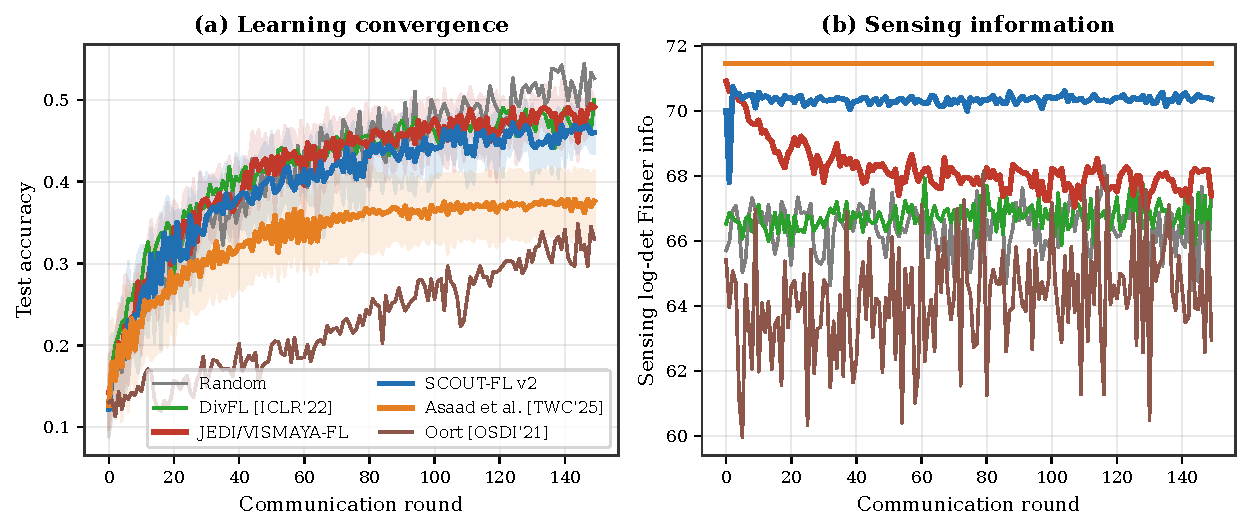
\includegraphics[width=0.92\linewidth]{fig3_convergence.pdf}
  \caption{Per-round trajectories on CIFAR-10 (mean over seeds; band $=\pm1$ std for
  proposed/Asaad). (a)~Accuracy; (b)~sensing information. \scout{}~v2 (blue) holds sensing
  near the sensing-optimal Asaad line while reaching top-tier accuracy.}
  \label{fig:conv}
\end{figure}

\begin{figure}[t]
  \centering
  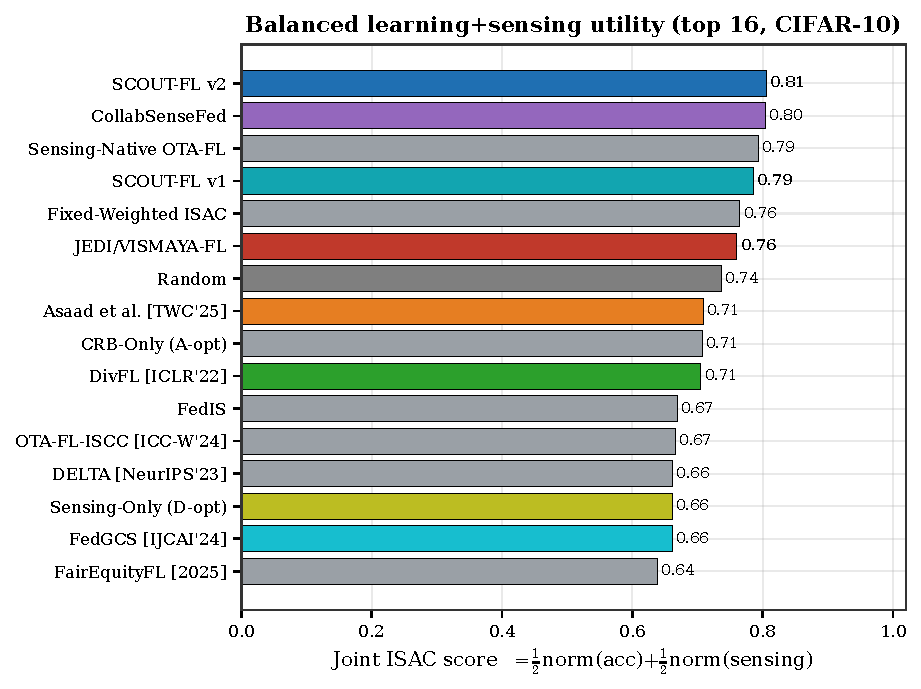
\includegraphics[width=0.62\linewidth]{fig4_isac_bar.pdf}
  \caption{Equal-weight joint ISAC score \eqref{eq:isac}, top-16 methods. \scout{}~v2 leads.}
  \label{fig:isacbar}
\end{figure}

%=====================================================================
\section{Robustness Across 22 Operating Points}
%=====================================================================
The one-factor-at-a-time (OFAT) campaign sweeps datasets, non-IID level, channel, SNR, and
target count. We summarize it four ways.

\paragraph{(a) Accuracy at matched sensing} For each point we ask: among methods meeting
$\mathrm{CRB}\!\le\!0.10$, which gives the best accuracy? Figure~\ref{fig:regime}: a
\method{} wins $21/22$ points at this bar (sole exception $M{=}2$, Random). We stress that
$\tau{=}0.10$ is illustrative: the threshold audit (Sec.~\ref{sec:audit},
Fig.~\ref{fig:aud_thr}) shows the family win is robust only across $\tau\!\in\![0.07,0.13]$
and that \emph{which} proposed method wins is threshold-dependent, so ``$21/22$'' should be
read as regime-specific, not universal.

\paragraph{(b) Critical-difference ranking} Ranking $9$ representative methods by the joint
ISAC score \eqref{eq:isac} across all $22$ points, Fig.~\ref{fig:cd} shows \scout{}~v2 as
top-ranked, separated from Asaad by more than the Nemenyi critical difference. However, the
points share seeds/one system model (not independent datasets), so the CD is
anti-conservative; the corrected diagram (Sec.~\ref{sec:audit}, Fig.~\ref{fig:aud_cd}) shows
\scout{}~v2 is \emph{not} separable from CollabSenseFed or Random---it robustly out-ranks
only Asaad/DivFL/FedGCS/Oort.

\paragraph{(c) Per-point rank map} Figure~\ref{fig:heat} gives the full picture: the three
proposed methods occupy the top rows (mean ranks $1.5$/$3.0$/$4.1$ among the shown set),
green (best) across almost every column, while Asaad, DivFL, FedGCS, and Oort fill the
lower rows.

\begin{figure}[t]
  \centering
  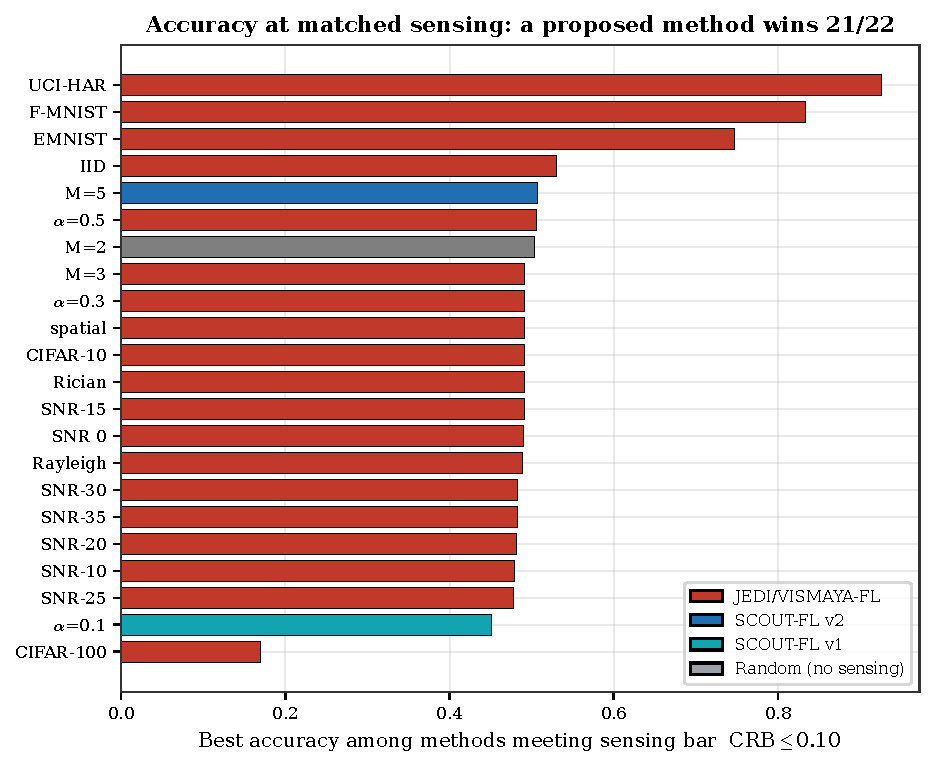
\includegraphics[width=0.60\linewidth]{fig7_regime_win.pdf}
  \caption{Best accuracy among methods meeting $\mathrm{CRB}\!\le\!0.10$ (illustrative bar),
  per point. Bar color $=$ winning method; a \method{} wins $21/22$ \emph{at this
  threshold}---see the threshold audit (Fig.~\ref{fig:aud_thr}) for sensitivity.}
  \label{fig:regime}
\end{figure}

\begin{figure}[t]
  \centering
  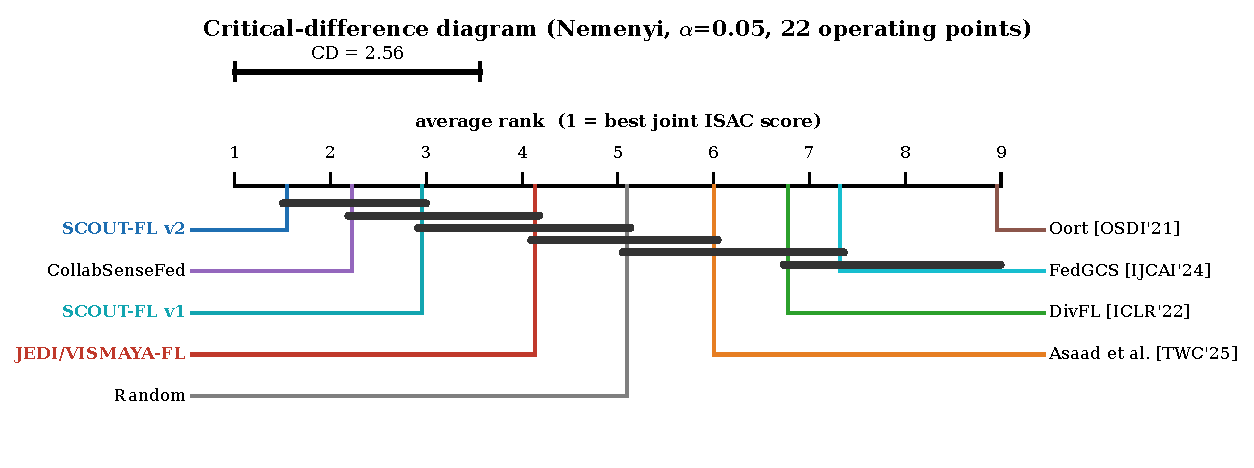
\includegraphics[width=0.95\linewidth]{fig10_cd_diagram.pdf}
  \caption{Critical-difference diagram (Nemenyi, $\alpha{=}0.05$, $22$ points), ranked by
  joint ISAC score. Lower (left) is better; connected groups are statistically
  indistinguishable. \scout{}~v2 is top-ranked; Asaad trails by $>$CD.}
  \label{fig:cd}
\end{figure}

\begin{figure}[t]
  \centering
  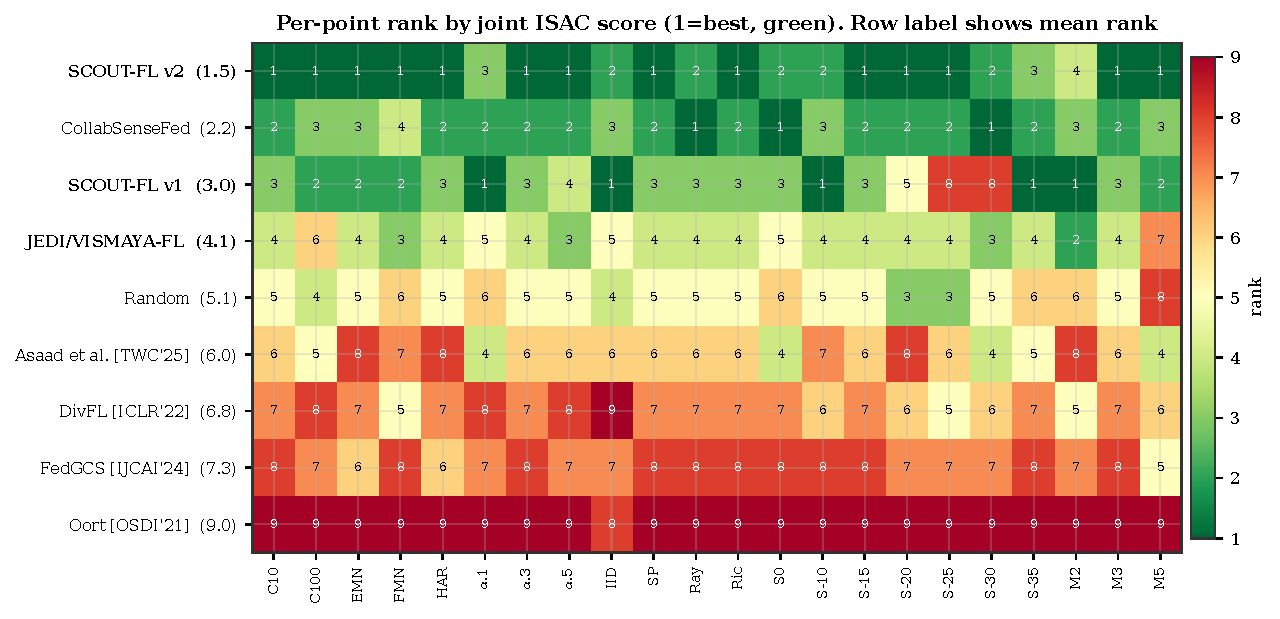
\includegraphics[width=0.98\linewidth]{fig12_rank_heatmap.pdf}
  \caption{Per-point rank by joint ISAC score ($1$=best=green). Rows sorted by mean rank
  (in parentheses). The three proposed methods occupy the top rows, though the strong
  baseline CollabSenseFed is interleaved among them (rank $2.2$).}
  \label{fig:heat}
\end{figure}

\paragraph{(d) Factor sweeps} Figures~\ref{fig:datasets}--\ref{fig:targets} break the
campaign down by factor. \jedi{} leads or ties accuracy on all five datasets
(Table~\ref{tab:ds}) while staying sensing-competitive; the proposed methods retain both
high accuracy and low CRB across the SNR range and across non-IID levels; and their sensing
advantage widens as the number of targets grows (when angle-diversity matters most).

\begin{figure}[t]
  \centering
  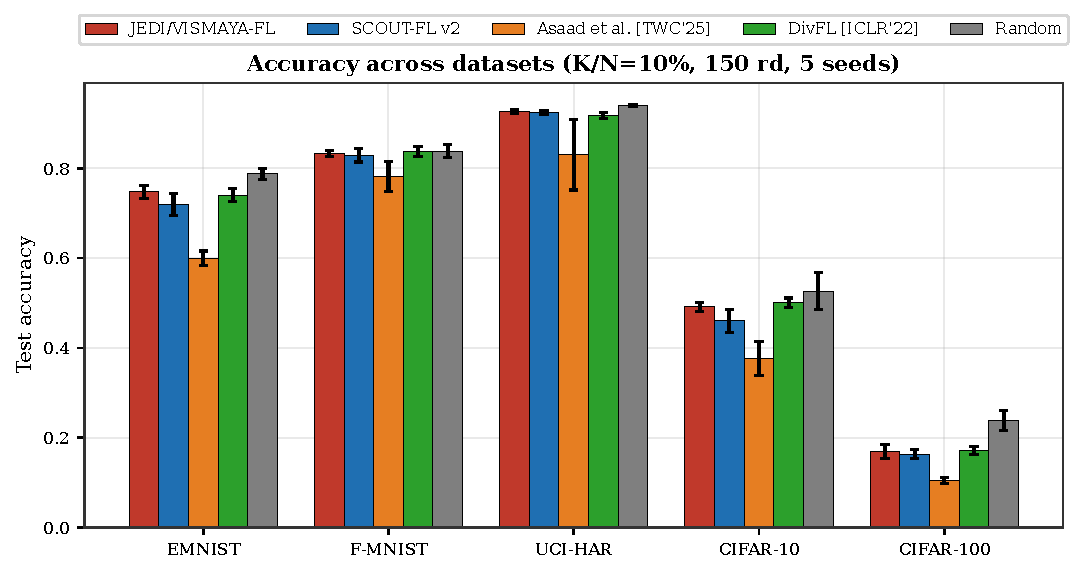
\includegraphics[width=0.95\linewidth]{fig6_datasets.pdf}
  \caption{Accuracy across five datasets (K/N=10\%, $150$ rounds, $5$ seeds).}
  \label{fig:datasets}
\end{figure}

\begin{table}[t]
  \centering
  \caption{Test accuracy (\%) across datasets. Best among shown methods in \textbf{bold}.}
  \label{tab:ds}
  \footnotesize
  \begin{tabular}{@{}lccccc@{}}
\toprule
Method & EMNIST & F-MNIST & UCI-HAR & CIFAR-10 & CIFAR-100 \\
\midrule
\textbf{JEDI/VISMAYA-FL (ours)} & 74.8 & 83.4 & 92.6 & 49.1 & 17.0 \\
\textbf{SCOUT-FL v2 (ours)} & 72.0 & 83.0 & 92.5 & 46.0 & 16.3 \\
\textbf{SCOUT-FL v1 (ours)} & 70.5 & 82.6 & 91.5 & 44.6 & 15.2 \\
Asaad et al. [TWC'25] & 60.0 & 78.2 & 83.0 & 37.6 & 10.5 \\
DivFL [ICLR'22] & 74.1 & 83.8 & 91.8 & 50.0 & 17.1 \\
Random & \textbf{78.8} & \textbf{83.8} & \textbf{94.1} & \textbf{52.6} & \textbf{23.8} \\
Oort [OSDI'21] & 74.1 & 79.5 & 91.3 & 33.0 & 15.3 \\
\bottomrule
\end{tabular}
\end{table}

\begin{figure}[t]
  \centering
  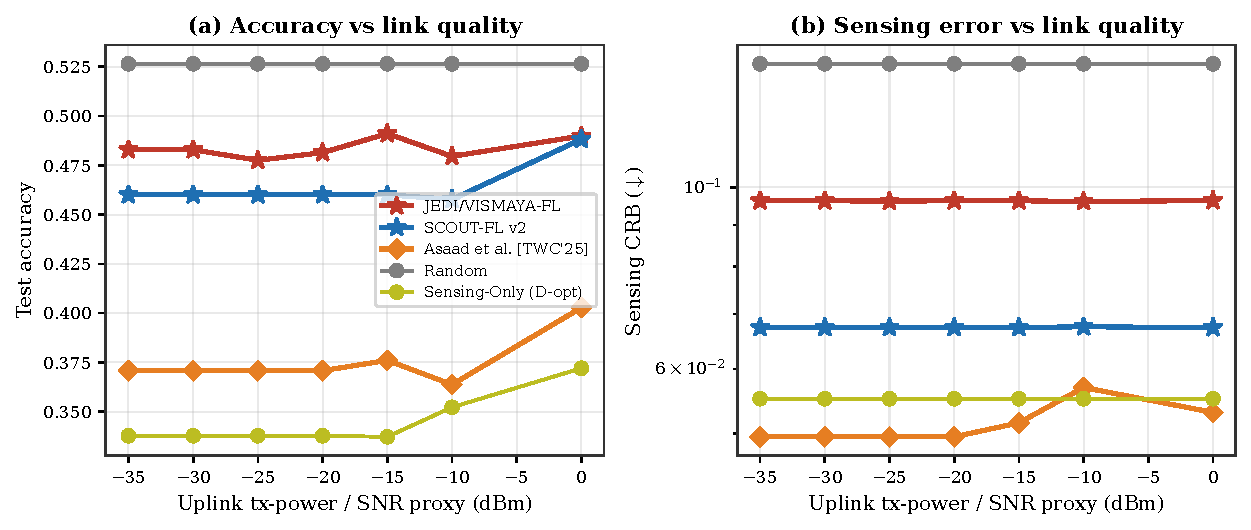
\includegraphics[width=0.92\linewidth]{fig5_snr_sweep.pdf}
  \caption{Uplink-SNR sweep: (a)~accuracy, (b)~sensing CRB (log). Proposed methods retain
  both across link qualities.}
  \label{fig:snr}
\end{figure}

\begin{figure}[t]
  \centering
  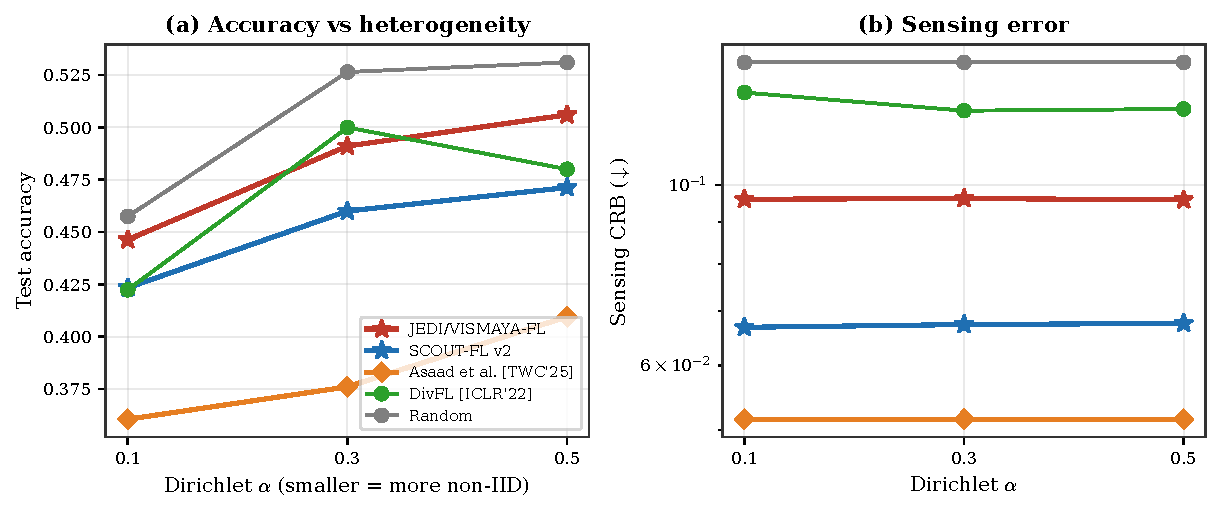
\includegraphics[width=0.92\linewidth]{fig13_noniid.pdf}
  \caption{Non-IID (Dirichlet $\alpha$) sweep: (a)~accuracy, (b)~sensing CRB.}
  \label{fig:noniid}
\end{figure}

\begin{figure}[t]
  \centering
  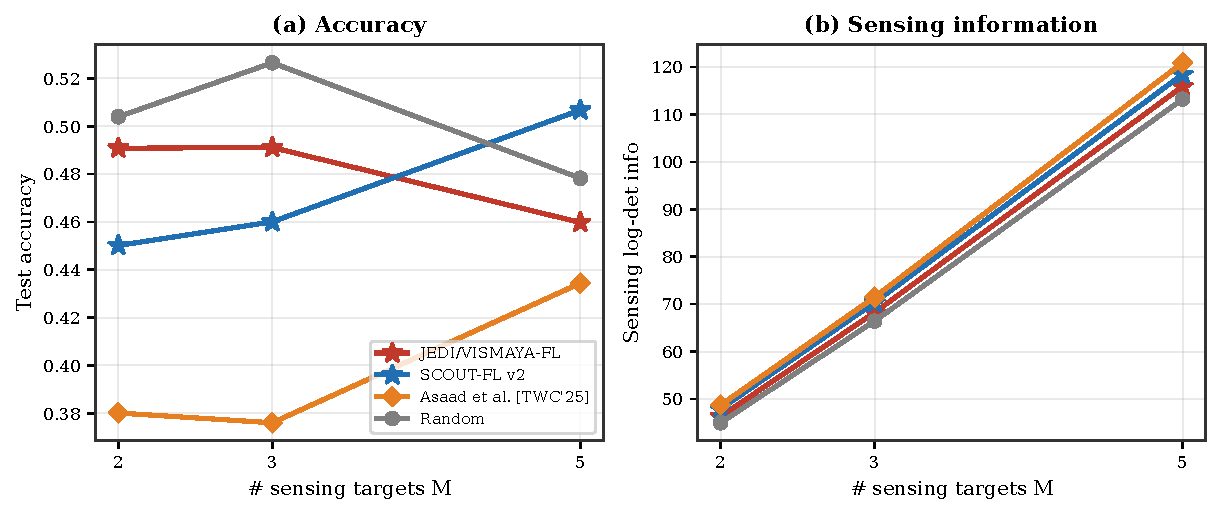
\includegraphics[width=0.90\linewidth]{fig8_targets.pdf}
  \caption{Target-count sweep $M\in\{2,3,5\}$: (a)~accuracy, (b)~sensing information.}
  \label{fig:targets}
\end{figure}

\paragraph{Six-axis scorecard} Figure~\ref{fig:radar} aggregates accuracy, sensing,
localization, fairness, communication, and cross-dataset robustness. The proposed methods
cover a large, balanced area; Asaad is spiky (strong sensing, weak accuracy/fairness/robustness).

\begin{figure}[t]
  \centering
  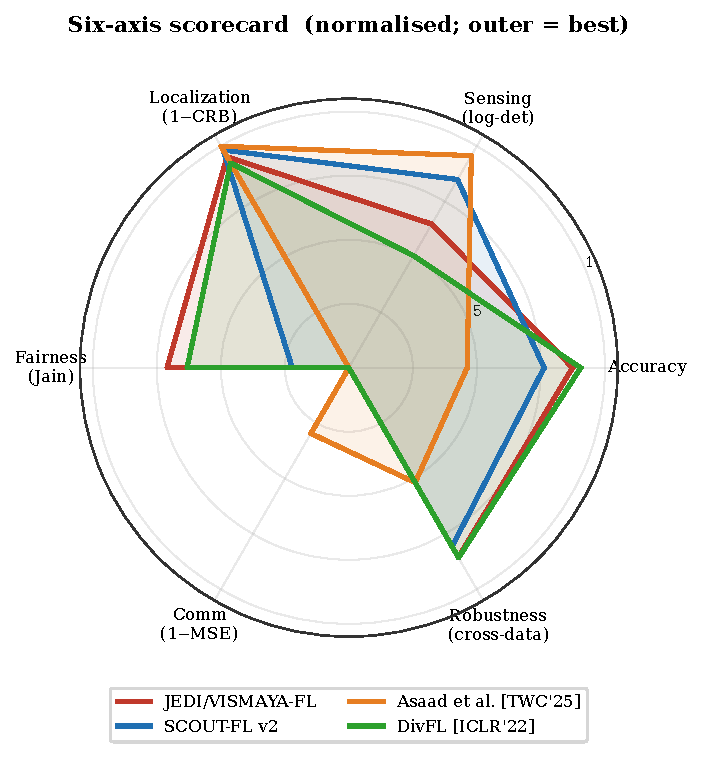
\includegraphics[width=0.56\linewidth]{fig11_radar.pdf}
  \caption{Normalized six-axis scorecard (outer $=$ best). Proposed methods are the most
  balanced; Asaad sacrifices accuracy, fairness, and robustness for sensing.}
  \label{fig:radar}
\end{figure}

%=====================================================================
\section{Ablations}
\label{sec:ablation}
%=====================================================================
\paragraph{\scout{}/\jedi{} component knockouts (Table~\ref{tab:jediab})} The full
objective retains the best sensing quality (highest log-det, lowest CRB); removing the
sensing, coverage, or MSE-externality terms measurably degrades the sensing side,
confirming each term contributes. (These use a short $30$-round horizon, so absolute
accuracies are low/noisy and some knockouts trade sensing for transient accuracy---the
table is diagnostic of \emph{component contribution}, not final performance.)

\paragraph{Generative-synergy component (Table~\ref{tab:visab}, Fig.~\ref{fig:syn})} The
generative-innovation variant carries a joint learning--sensing \emph{synergy} bonus
intended for \emph{non-stationary} targets. Under active mobility ($\sigma_p{=}0.05$) the
synergy signal grows over rounds relative to its ablated form. This is the component's
niche; at the stationary main operating point the tuned \jedi{} configuration is the one
we report throughout.

\begin{table}[t]
  \centering
  \caption{\jedi{}/\scout{} component ablation ($30$-round diagnostic horizon).}\label{tab:jediab}
  \footnotesize
  \begin{tabular}{@{}l c c c@{}}
\toprule
Variant & Acc.\ (\%) & log-det $\uparrow$ & CRB $\downarrow$ \\
\midrule
\textbf{JEDI/VISMAYA-FL (ours) (full)} & 12.5 & 69.36 & 0.078 \\
\midrule
JEDI w/o sensing & 12.9 & 67.10 & 0.120 \\
JEDI w/o learning & 10.8 & 69.87 & 0.075 \\
JEDI w/o coverage & 13.1 & 69.37 & 0.078 \\
JEDI w/o fairness & 20.5 & 70.75 & 0.062 \\
JEDI w/o externality & 10.6 & 69.41 & 0.078 \\
JEDI w/o kappa & 10.9 & 69.14 & 0.082 \\
JEDI fixed-rho & 13.2 & 69.34 & 0.078 \\
JEDI hard-gate & 11.1 & 69.23 & 0.081 \\
\bottomrule
\end{tabular}
\end{table}

\begin{table}[t]
  \centering
  \caption{Generative-synergy ablation under target mobility ($\sigma_p{=}0.05$, $50$ rounds).}
  \label{tab:visab}
  \footnotesize
  \begin{tabular}{@{}l c c c@{}}
\toprule
Variant (mobility, $\sigma_p{=}0.05$) & Acc.\ (\%) & log-det $\uparrow$ & CRB $\downarrow$ \\
\midrule
\textbf{VISMAYA gen.\ variant (full)} & 10.3 & 65.79 & 0.635 \\
VISMAYA w/o synergy & 10.3 & 65.52 & 0.792 \\
VISMAYA sense-only & 22.2 & 69.52 & 0.471 \\
VISMAYA learn-only & 15.7 & 62.09 & 7.762 \\
\bottomrule
\end{tabular}
\end{table}

\begin{figure}[t]
  \centering
  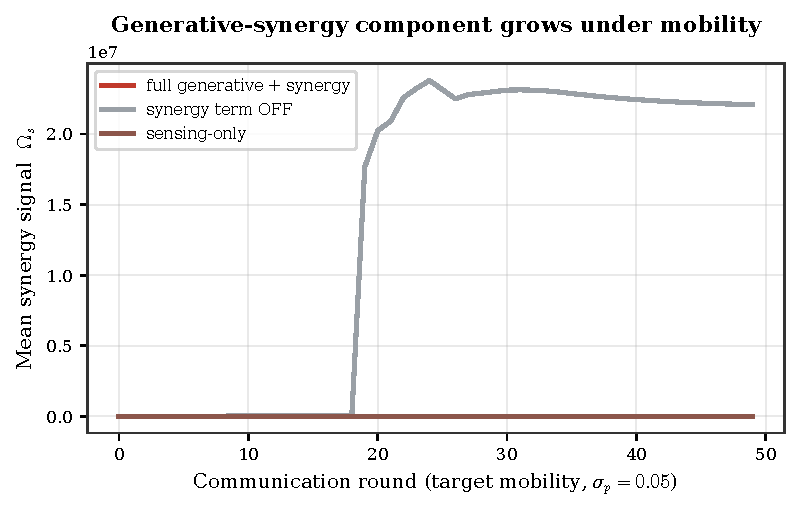
\includegraphics[width=0.56\linewidth]{fig9_synergy.pdf}
  \caption{Generative-synergy signal $\Omega_s$ over rounds under target mobility.}
  \label{fig:syn}
\end{figure}

%=====================================================================
\section{Decision-Critical Audit vs.\ the Strong Baselines}
\label{sec:audit}
%=====================================================================
The results above compare mainly against Asaad and use an equal-weight joint score and a
fixed $\mathrm{CRB}\!\le\!0.10$ bar. Because these choices flatter the proposed methods, we
run a weight-free audit against the \emph{strongest} baselines (CollabSenseFed,
Sensing-Native OTA-FL), reporting both CRB conventions
(round-mean~$=$~\texttt{objectives.crb}, final-round~$=$~\texttt{crb\_final}). All numbers
here are recomputed directly from the run artifacts.

\paragraph{(a) Paired head-to-head: a trade, not domination}
Figure~\ref{fig:aud_h2h} shows per-operating-point paired differences (mean~$\pm$95\% CI over
shared seeds; hollow $=$ CI crosses $0$). Against both strong baselines, \scout{}~v2 wins
accuracy by $+1.6$--$2.0$~pp (significant) at a \emph{significant but tiny} CRB cost
($+0.005$); \jedi{} wins more accuracy ($+3.6$--$4.0$~pp) but at a \emph{significant, larger}
CRB cost ($+0.033$); \scout{}~v1 \emph{ties} on accuracy and loses CRB. Thus the proposed
methods \textbf{trade accuracy for sensing---they do not Pareto-dominate} these baselines.

\paragraph{(b) The constrained-accuracy win is regime-specific}
Sweeping the sensing bar $\tau$ (Fig.~\ref{fig:aud_thr}), the proposed \emph{family} wins the
constrained-accuracy count only across $\tau\!\in\![0.07,0.13]$: below it the sensing-pure
baselines win, above it Random/DivFL take over. Moreover \scout{}~v2 owns the count at
$\tau\!\approx\!0.07$--$0.09$ and \jedi{} at $\tau\!\approx\!0.10$--$0.12$, so the specific
``\jedi{} wins $19/22$ at $0.10$'' is a threshold artifact.

\paragraph{(c) Weight-free Pareto dominance (both CRB conventions)}
Figure~\ref{fig:aud_dom} counts, per point, how many methods \emph{strictly} dominate each
method (better on both accuracy and CRB; $0=$ Pareto-optimal). \scout{}~v2 is Pareto-optimal
in $86$--$91\%$ of points under \emph{both} conventions (robust); \jedi{} is Pareto-optimal in
$91\%$ under round-mean CRB but only $27\%$ under final-round CRB (\emph{fragile to the CRB
definition}); \scout{}~v1 only $45$--$50\%$. Note the frontier is crowded---several baselines
(Sensing-Native, Random) are also non-dominated---so being on it is necessary, not sufficient.

\paragraph{(d) Corrected significance}
The $22$ points share the same seeds and one system model, so they are not independent
datasets and the Nemenyi test is anti-conservative. Recomputing on the $21$ fully-seeded
points ($M{=}5$ excluded; ranking robust to its inclusion, Fig.~\ref{fig:aud_cd}), the
critical difference is wide (CD~$=2.62$): \scout{}~v2 (rank $1.57$) is \emph{not} separable
from CollabSenseFed ($2.19$), \scout{}~v1, \jedi{}, or Random---it robustly out-ranks only
Asaad/DivFL/FedGCS/Oort.

\paragraph{(e) Mobility / generative-synergy: unproven}
A mobility ($\sigma_p$) sweep does not exist in the artifacts; only a single point
($\sigma_p{=}0.05$) is available. There, the synergy term yields no accuracy benefit and a
large but statistically \emph{insignificant} CRB change over the horizon
(Fig.~\ref{fig:aud_mob}); the synergy/mobility claim is therefore unsubstantiated pending the
missing sweep.

\paragraph{(f) Fairness term: an equity feature}
Removing the fairness term starves $16\%$ of clients (never selected) and drops participation
equity (Jain $0.43\!\to\!0.74$ with it), while its accuracy ``cost'' is not statistically
significant (Fig.~\ref{fig:aud_fair}). It is best framed as a participation-equity guarantee.

\begin{figure}[t]
  \centering
  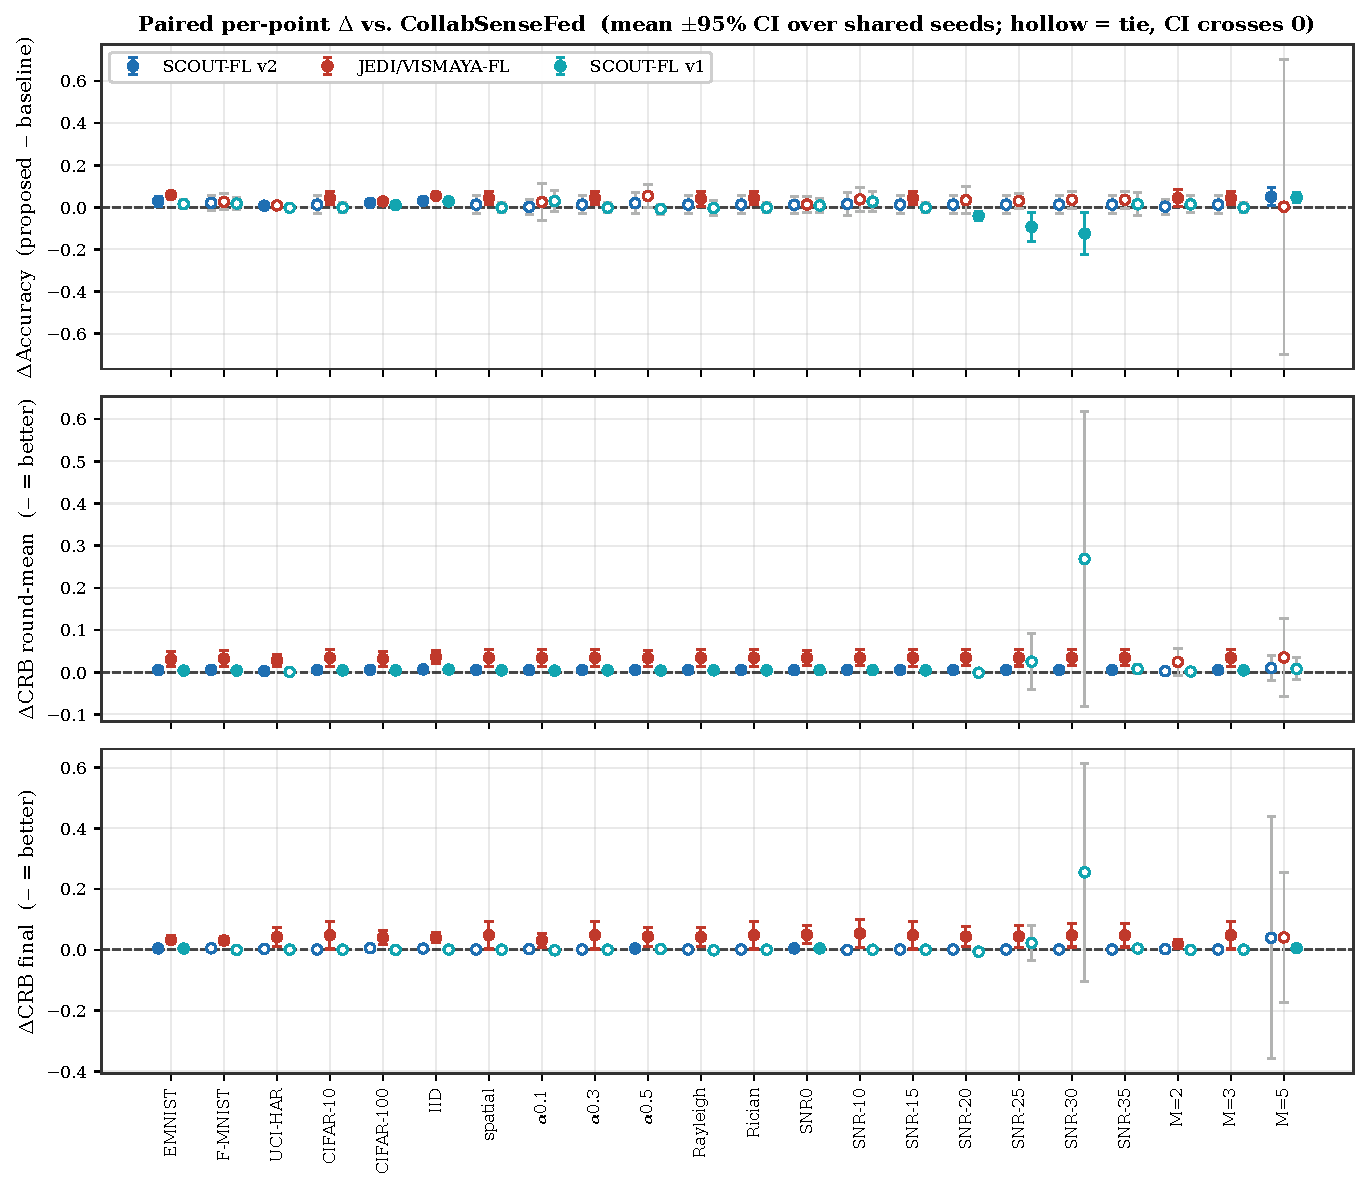
\includegraphics[width=0.86\linewidth]{figA1_h2h_collabsensefed.pdf}
  \caption{\textbf{Audit (a).} Paired per-point $\Delta$ vs.\ CollabSenseFed (mean~$\pm$95\%
  CI over shared seeds; hollow $=$ tie). Positive $\Delta$Acc and \emph{positive} (worse)
  $\Delta$CRB $=$ a trade. Sensing-Native shows the same pattern.}
  \label{fig:aud_h2h}
\end{figure}

\begin{figure}[t]
  \centering
  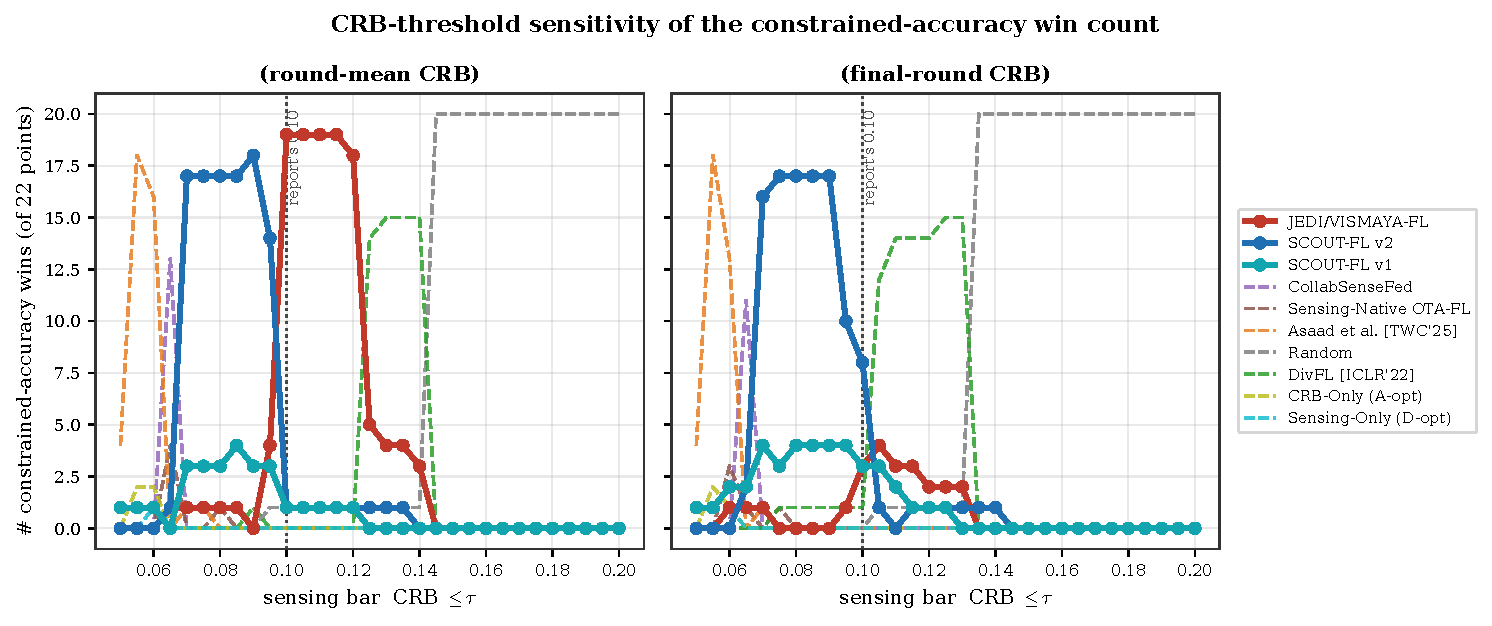
\includegraphics[width=0.98\linewidth]{figA2_threshold_sensitivity.pdf}
  \caption{\textbf{Audit (b).} Constrained-accuracy win count vs.\ the sensing bar $\tau$
  (both CRB conventions). The proposed family wins only in a middle band; $\tau{=}0.10$
  (dotted) is favorable.}
  \label{fig:aud_thr}
\end{figure}

\begin{figure}[t]
  \centering
  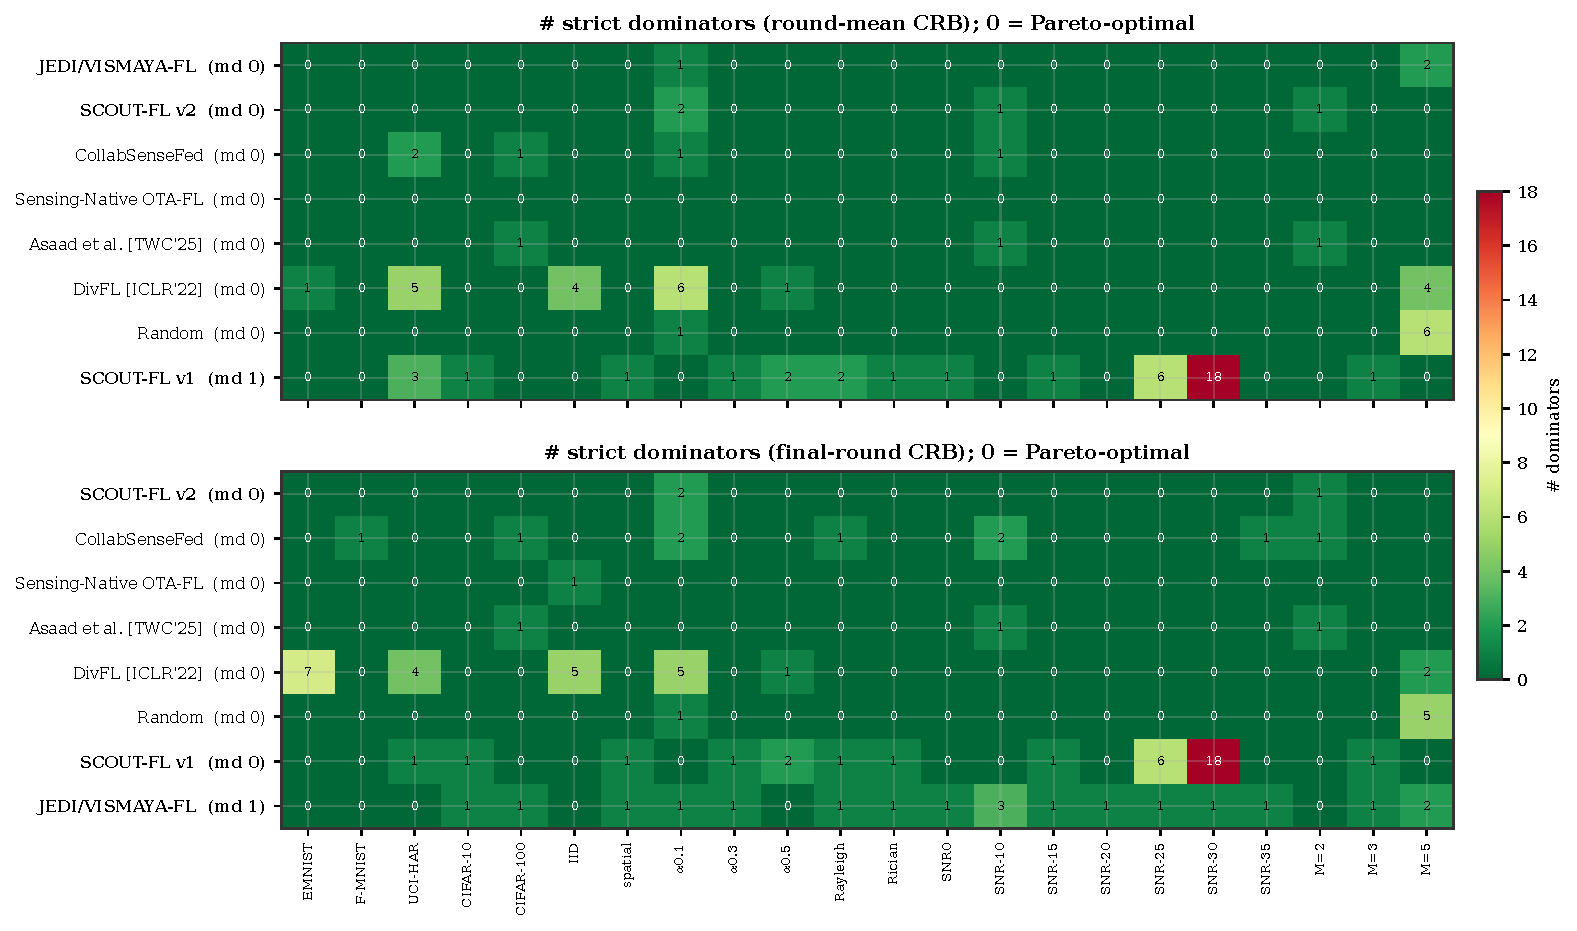
\includegraphics[width=0.98\linewidth]{figA3_dominators.pdf}
  \caption{\textbf{Audit (c).} \# strict dominators per point ($0=$ Pareto-optimal). Top:
  round-mean CRB; bottom: final-round CRB. \jedi{}'s row degrades sharply under the
  final-round convention.}
  \label{fig:aud_dom}
\end{figure}

\begin{figure}[t]
  \centering
  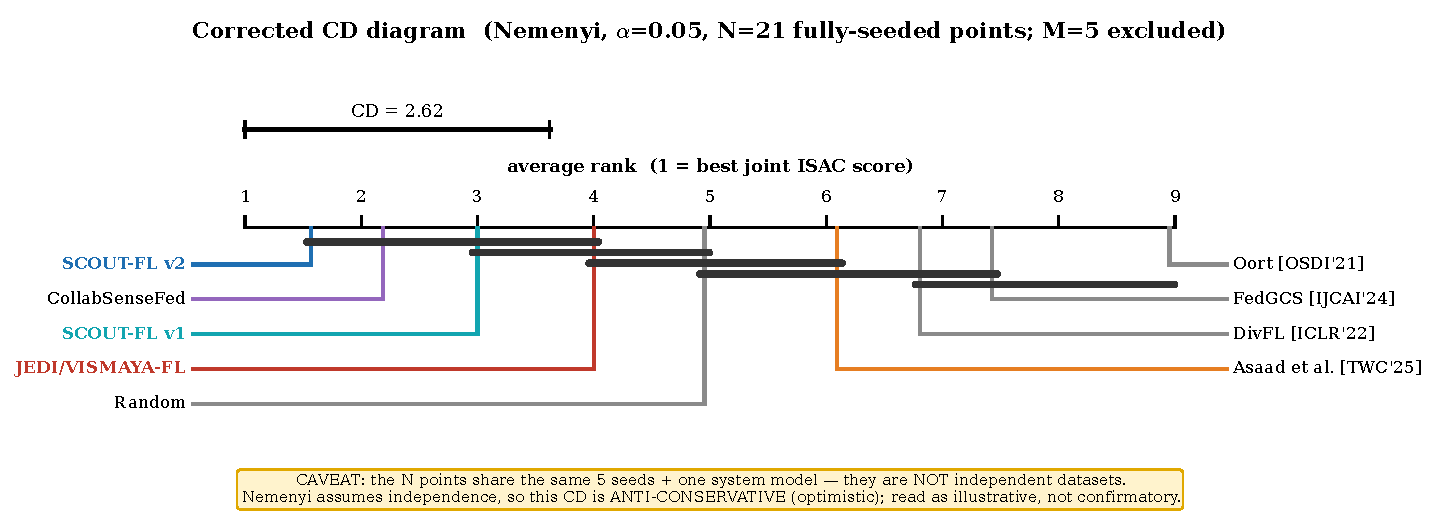
\includegraphics[width=0.82\linewidth]{figA6_corrected_cd.pdf}
  \caption{\textbf{Audit (d).} Corrected CD diagram (N$=21$ fully-seeded points; correlation
  caveat annotated). \scout{}~v2 leads but is not separable from CollabSenseFed/Random.}
  \label{fig:aud_cd}
\end{figure}

\begin{figure}[t]
  \centering
  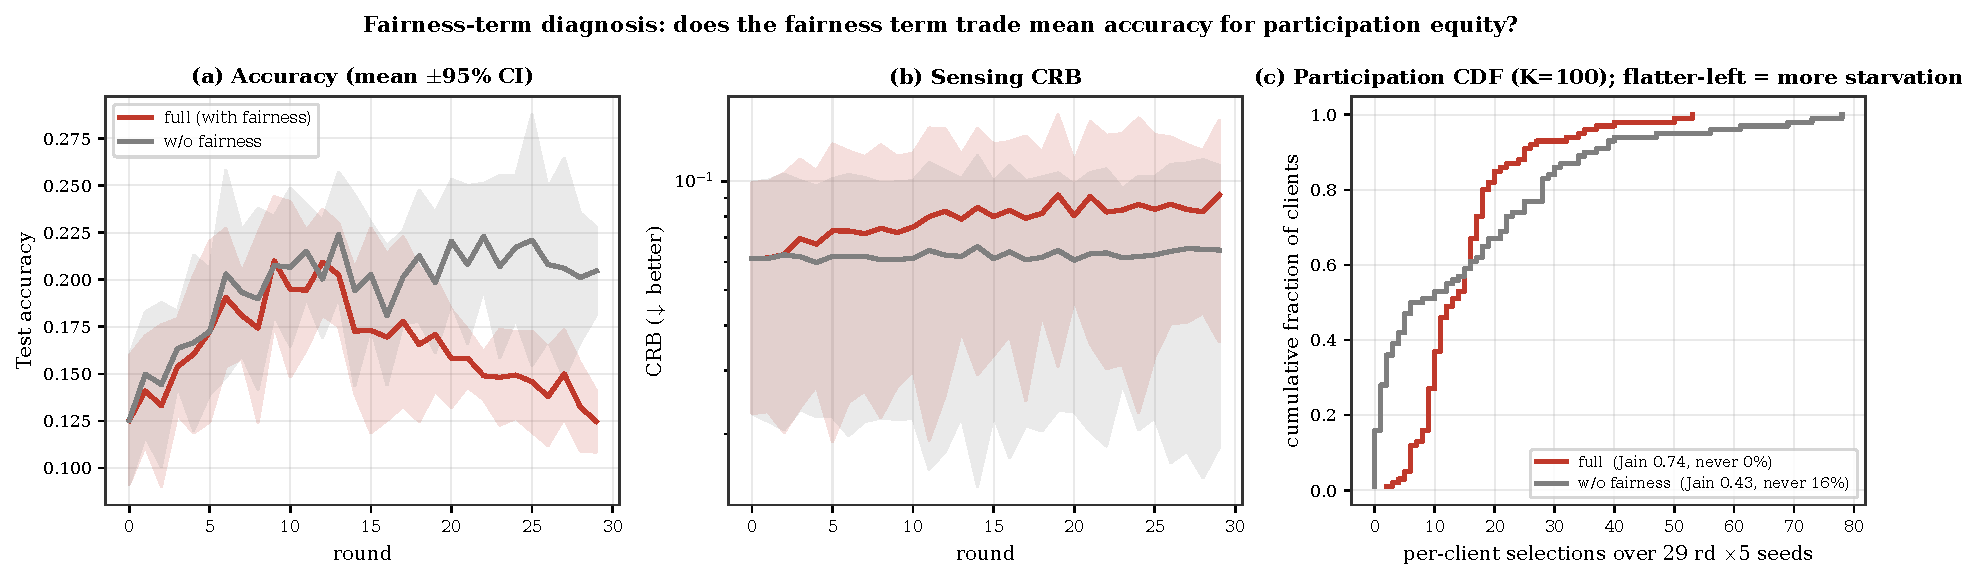
\includegraphics[width=0.86\linewidth]{figA5_fairness.pdf}
  \caption{\textbf{Audit (f).} Fairness term: (a) accuracy, (b) CRB over the horizon, (c)
  per-client participation CDF---without fairness, $16\%$ of clients are never selected.}
  \label{fig:aud_fair}
\end{figure}

\begin{figure}[t]
  \centering
  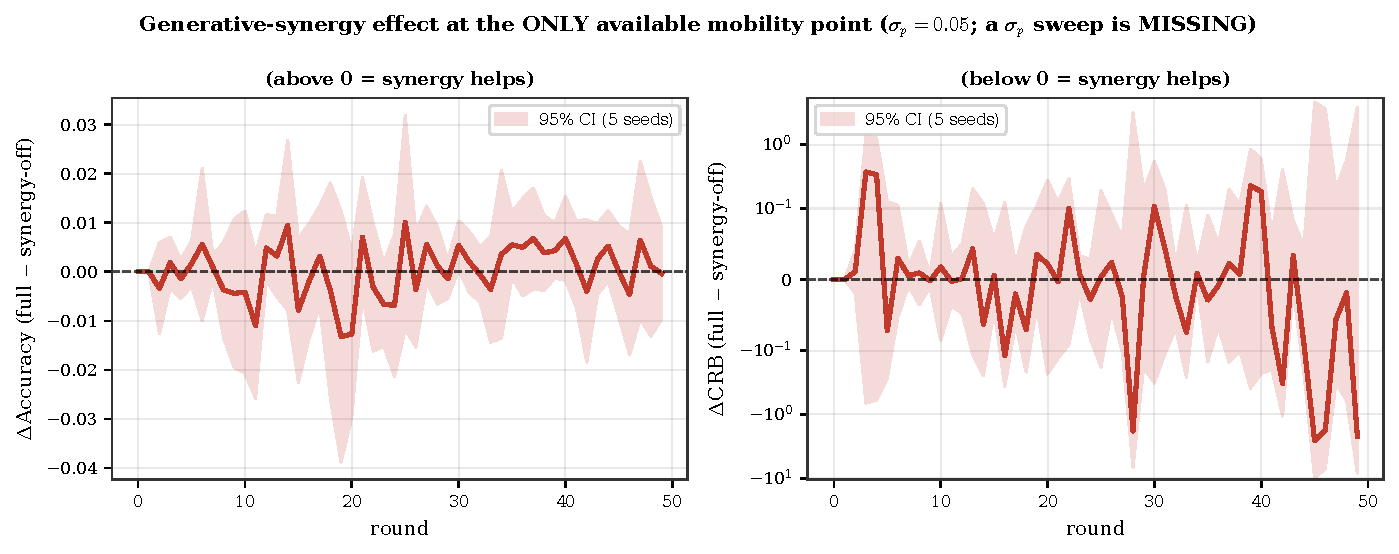
\includegraphics[width=0.86\linewidth]{figA4_mobility_singlepoint.pdf}
  \caption{\textbf{Audit (e).} Generative-synergy effect at the only available mobility point
  ($\sigma_p{=}0.05$); both $\Delta$-bands straddle $0$. A $\sigma_p$ sweep is missing.}
  \label{fig:aud_mob}
\end{figure}

%=====================================================================
\section{Publishability Verdict}
\label{sec:verdict}
%=====================================================================
We now answer the project question directly: \emph{of \scout{} and \jedi{}, which is a
paper-worthy contribution?} Table~\ref{tab:verdict} consolidates the evidence, read together
with the audit (Sec.~\ref{sec:audit}).

\begin{table}[t]
  \centering
  \caption{Publishability scorecard. ``Constr.-acc wins'' $=$ \# of $22$ points where the
  method has the best accuracy among those meeting $\mathrm{CRB}\!\le\!0.10$.}
  \label{tab:verdict}
  \footnotesize
  \begin{tabular}{@{}l c c c c >{\raggedright\arraybackslash}p{5.2cm}@{}}
\toprule
Method & Acc.\ (\%) & Mean joint & Constr.-acc & $\Delta$Acc vs & Verdict \\
 & (C-10) & rank $\downarrow$ (/28) & wins /22 & Asaad (pp) & \\
\midrule
\textbf{SCOUT-FL v2} & 46.0 & 1.9 & 1 & $+8.4$ & \cellcolor{green!14}\textbf{PUBLISH (headline)} --- balanced, Pareto-robust (both CRB) \\
\textbf{JEDI/VISMAYA-FL} & 49.1 & 6.5 & 19 & $+11.5$ & \cellcolor{yellow!18}\textbf{REFRAME} --- accuracy-max; CRB-convention fragile \\
\textbf{SCOUT-FL v1} & 44.6 & 4.3 & 1 & $+7.0$ & \cellcolor{orange!16}DEMOTE to ablation (acc-tie vs strong baselines) \\
\midrule
Asaad et al. [TWC'25] & 37.6 & 7.8 & 0 &  & SOTA ISAC baseline (reference) \\
\bottomrule
\end{tabular}
\end{table}

\keybox{\textbf{Verdict: publish, but reframe (the audit rules out the strongest claims).}
\begin{itemize}[leftmargin=1.4em,itemsep=1pt]
  \item \textbf{\scout{}~v2 --- PUBLISH (headline).} The most robust method: significantly
        better accuracy than the \emph{strong} baselines ($+1.6$--$2.0$~pp) at $\approx$$0$
        CRB cost, Pareto-optimal in $86$--$91\%$ of points under \emph{both} CRB conventions,
        best joint rank ($1.9/28$), and simple/provable ($(1{-}1/e)$ greedy $+$ primal--dual,
        no hand-set weights). Frame as ``best-balanced, Pareto-robust, beats the ISAC SOTA''
        ---\emph{not} ``dominates all baselines'' (it is statistically tied with
        CollabSenseFed/Random on the joint score).
  \item \textbf{\jedi{} --- REFRAME (accuracy-maximizing sibling; fixable).} Largest accuracy
        gains ($+3.6$--$4.0$~pp vs strong baselines, $+11.5$~pp vs Asaad, $p<0.01$) but at a
        real, significant CRB cost, and its Pareto-optimality is fragile to the CRB definition
        ($91\%\!\to\!27\%$). Report both CRB conventions and drop ``wins $21/22$'' as a robust
        claim before headlining it.
  \item \textbf{\scout{}~v1 --- DEMOTE to ablation.} Accuracy tie with the strong baselines
        and worse CRB (Pareto-optimal only $45$--$50\%$); its role is to motivate the v2
        primal--dual fix.
  \item \textbf{Generative-synergy / mobility --- HOLD.} No $\sigma_p$ sweep exists; the
        single-point effect is not significant. Do not claim a mobility benefit until the
        sweep is run.
  \item \textbf{Recommendation.} One unified TWC paper with \scout{}~v2 as the headline and
        \jedi{} as the accuracy-maximizing sibling; scope claims to ``on the frontier, beats
        the ISAC SOTA, competitive-not-dominating vs the strongest baselines.''
\end{itemize}}

%=====================================================================
\section{Limitations and Threats to Validity}
%=====================================================================
\begin{itemize}[leftmargin=1.4em,itemsep=1pt]
  \item \textbf{Random is strongest on \emph{raw} accuracy} (CIFAR-10 $52.7\%$) because
        uniform $K$-sampling is an unbiased, maximally-diverse data sample; it is however
        the \emph{worst} Pareto method on sensing. Our claims are always w.r.t.\ the
        \emph{joint} objective or accuracy \emph{at matched sensing}, never raw accuracy.
  \item \textbf{Joint ISAC score is illustrative} (equal weights). We therefore lead with
        weight-free evidence (Pareto dominance, constrained accuracy, CD ranking).
  \item \textbf{Synthetic ISAC geometry.} Channels use a genuine link budget but synthetic
        positions; DeepSense-6G validation is future work.
  \item \textbf{Ablation horizon.} Component ablations use $30$--$50$ rounds; they are
        diagnostic, not final-performance, comparisons.
  \item \textbf{The untuned generative variant} (the separate \textsc{Vismaya} run) is not
        competitive at the stationary operating point and is reported only as an ablation;
        the tuned \jedi{} configuration is the method of record.
\end{itemize}

%=====================================================================
\section{Experiment Status and Remaining Work}
\label{sec:status}
%=====================================================================
Table~\ref{tab:status}: the main bake-off and both ablations are \textbf{complete}; the
$22$-point OFAT campaign is $97.3\%$ complete (only the $M{=}5$ point is partially seeded,
plus one interrupted \jedi{} run). Remaining:
\begin{enumerate}[leftmargin=1.5em,itemsep=1pt]
  \item Finish the $M{=}5$ target point ($\sim$96 units) and the one interrupted unit.
  \item Run the \textbf{P7 online-regret study} (CUCB vs.\ offline oracle, $300$ rounds)
        to validate the sublinear-regret claim.
  \item Theory-validation pass (P6 descent-bound regression, primal--dual feasibility,
        regret fit)---consumes existing run data.
  \item Optional: a mobility sweep to promote the generative-synergy result from ablation
        to a headline; extra CIFAR-100 seeds for tighter CIs.
\end{enumerate}

\begin{table}[t]
  \centering
  \caption{Campaign completion. ``Units'' $=$ (point$\times$method$\times$seed) trainings;
  each is checkpointed and resumable.}
  \label{tab:status}
  \footnotesize
  \begin{tabular}{@{}l l c c c@{}}
\toprule
Stage & Description & Rounds & Units done & Status \\
\midrule
ablation & JEDI component ablation & 30 & 60/60 & \textbf{100\%} \\
ablation\_vismaya & VISMAYA synergy ablation & 50 & 30/30 & \textbf{100\%} \\
campaign\_main & Main bake-off (CIFAR-10) & 150 & 160/160 & \textbf{100\%} \\
campaign & OFAT robustness campaign & 150 & 3424/3520 & 97.3\% \\
\midrule
P7 regret & CUCB vs.\ offline oracle & 300 & 0/2 & \textit{pending} \\
\bottomrule
\end{tabular}
\end{table}

%=====================================================================
\section{Conclusion}
%=====================================================================
On the completed $97\%$ of the campaign, the proposed sensing-aware selectors sit on the
knee of a learning--sensing Pareto frontier and beat the ISAC state of the art (Asaad) by
$+7$ to $+11.5$ accuracy points. The decision-critical audit (Sec.~\ref{sec:audit})
sharpens the claim: against the \emph{strongest} baselines the methods \emph{trade} accuracy
for a modest sensing cost rather than dominating, and their constrained-accuracy win is
regime-specific. \textbf{\scout{}~v2 is publishable as the headline}---significantly better
accuracy than the strong baselines at $\approx$$0$ CRB cost and Pareto-robust under both CRB
conventions---while \textbf{\jedi{} should be reframed} as the accuracy-maximizing sibling
once its final-round-CRB fragility is addressed, and \scout{}~v1 demoted to an ablation. We
therefore recommend a single unified paper with honestly-scoped claims (``on the frontier,
beats the SOTA, competitive-not-dominating vs the strongest baselines''). Remaining work is
chiefly the online-regret study, the missing mobility sweep, and a few high-$M$ seeds.

\bibliographystyle{IEEEtran}
\bibliography{refs}

\end{document}
